\documentclass[a4paper, 10pt, final, garamond]{book}
\usepackage{cours-preambule}
\graphicspath{{./figures/}}

\makeatletter
\renewcommand{\@chapapp}{Contr\^ole de connaissances}
\makeatother

% \toggletrue{student}
% \HideSolutionstrue

\begin{document}
\setcounter{chapter}{0}

\chapter{Optique~: miroirs et lentilles}

\begin{enumerate}[label=\sqenumi, leftmargin=10pt]
	\nitem{3} Pour un rayon passant d'un milieu d'indice $n_1$ à un milieu
	d'indice $n_2$, à quelle condition peut-on avoir réflexion limite~? Tracer un
	schéma d'une situation de réflexion totale. Déterminer l'angle de réflexion
	limite.
  \smallbreak
  \begin{isd}[righthand ratio=.3]
		\wsw{
			On peut avoir réflexion totale si $n_2 < n_1$.
			Soit $i_{\rm lim}$ l'angle d'incidence limite de réfraction, tel que
			$i_2 = \frac{\pi}{2}$. On a~:
			\begin{equation*}
				i_2 = \frac{\pi}{2} \Rightarrow \sin(i_2) = 1
			\end{equation*}
			Or, $n_2\sin(i_2) = n_1\sin(i_{\rm lim})$ d'après la loi de
			Snell-Descartes pour la réfraction. Ainsi,
			\begin{gather*}
				n_2 \underbrace{\cancel{\sin(i_2)}}_{=1} = n_1\sin(i_{\rm lim})
				\Leftrightarrow \frac{n_2}{n_1}          = \sin(i_{\rm lim})
				\Rightarrow i_{\rm lim}                  = \arcsin \left( \frac{n_2}{n_1} \right)
			\end{gather*}
		}
    \vspace*{-20pt}
		\tcblower
		\begin{center}
      \switch{
              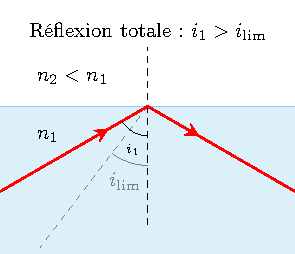
\includegraphics[width=\linewidth, draft=true]{refl_tot-3}
      }{
			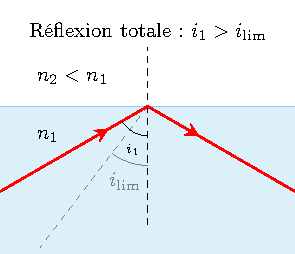
\includegraphics[width=\linewidth]{refl_tot-3}
      }
		\end{center}
	\end{isd}
  \nitem{3} Donnez, avec un schéma comportant le tracé des rayons, la relation
  de conjugaison d'un miroir plan. Que vaut son grandissement transversal~?
  Donnez, sans schéma, les relations de conjugaison des lentilles minces.
  \smallbreak
  \begin{isd}[righthand ratio=.2]
    \wsw{
      \begin{gather*}
        \tan(i) =
        \frac{\obar{\rm HI}}{\obar{\rm HA}} =
        \frac{\obar{\rm HI}}{-\obar{\rm HA'}} =
        \boxed{\obar{\rm HA'} = -\obar{\rm HA}}
        \qav
        \boxed{\gamma = +1}
      \end{gather*}
      et
      \[
        \boxed{ \frac{1}{\OFp} = \frac{1}{\OAp} - \frac{1}{\OA}}
        \qou
        \boxed{-f'^2 = \obar{\rm F'A'}\obar{\rm FA}}
      \]
    }
    \vspace*{-20pt}
    \tcblower
    \begin{center}
      \switch{
        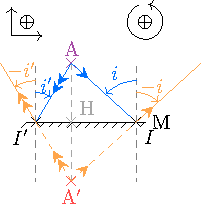
\includegraphics[width=\linewidth, draft=true]{mir_plan-obj_r}
      }{
        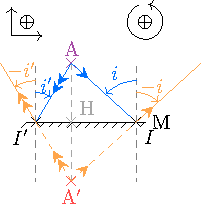
\includegraphics[width=\linewidth]{mir_plan-obj_r}
      }
      \label{fig:mir_plan-obj_r}
    \end{center}
  \end{isd}
  \nitem{4} Construisez les images dans les situations suivantes.
  \smallbreak
  \begin{center}
      \begin{tabular}{cc}
        \switch{
                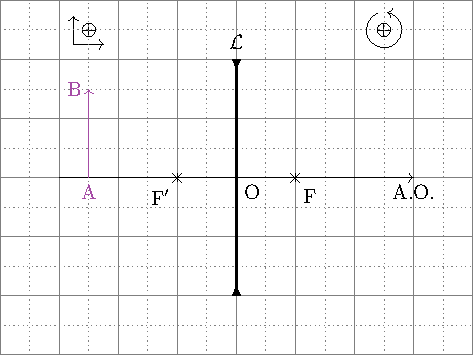
\includegraphics[width=.40\linewidth]{lent_div-constru_simple-plain}
        }{
        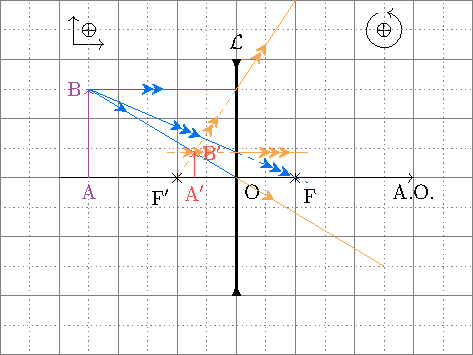
\includegraphics[width=.40\linewidth]{lent_div-constru_simple}
        }
    &
        \switch{
                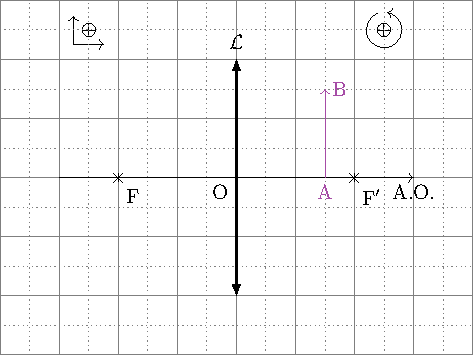
\includegraphics[width=.40\linewidth]{lent_conv-constru_after-plain}
        }{
        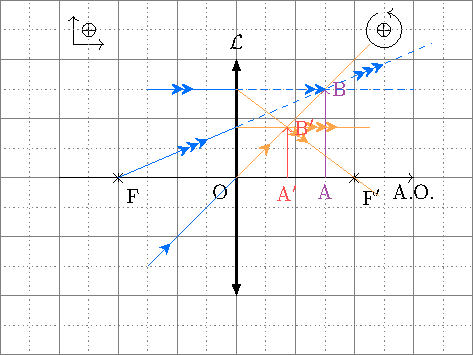
\includegraphics[width=.40\linewidth]{lent_conv-constru_after}
        }
    \\
        \switch{
                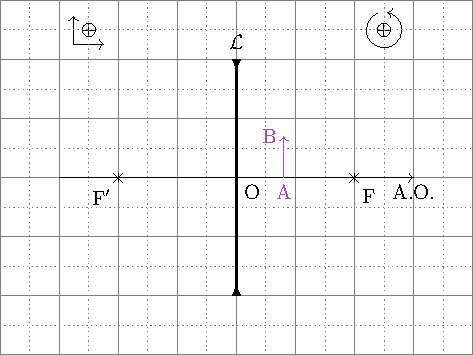
\includegraphics[width=.40\linewidth]{lent_div-constru_after_a-plain}
        }{
        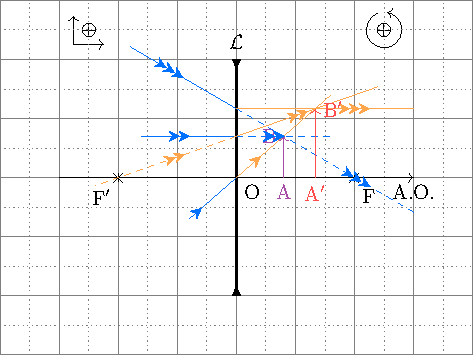
\includegraphics[width=.40\linewidth]{lent_div-constru_after_a}
        }
    &
        \switch{
                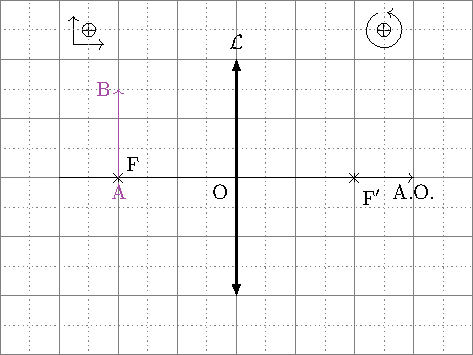
\includegraphics[width=.40\linewidth]{lent_conv-constru_F-plain}
        }{
        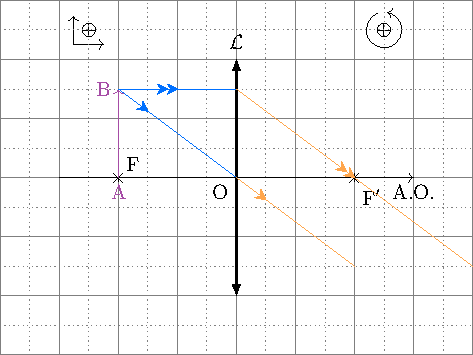
\includegraphics[width=.40\linewidth]{lent_conv-constru_F}
        }
    \end{tabular}
  \end{center}
\end{enumerate}

\end{document}
